% TODO: GENERAL CHECKUP NEEDED

\section{Shelled Kin}
\begin{linenumbers}
\textit{I caught a big fish.}

\textit{Now I search for a good friend}

\textit{To share my lunch with.}

\hspace*{\fill} --- Tortle haiku.

The shelled kin are a species native to the outer lands.
Also known as tortles, they have gracefully adapted to their lives in Yuadrem, able to start a new life in the land ravaged by the schism, and it is very common to see the rustic tortle villages in the coasts of the beryl sea and many of the eastern shores of the continent.
% The shelled kin or tortles are a species native to the outer lands which, unlike umans, don't seem to be hunted by the strange creatures from this place, and remain unaffected by the forbidden lands.

What many tortles consider a simple life, others might call a life of adventure.
Tortles are born near sandy coastlines, but as soon as they're able to walk on two legs, they turn into nomad survivalists eager to explore the wilderness, experience its many wonders, put their skills to the test, and make new acquaintances.

\begin{figure}[!b]
    \centering
    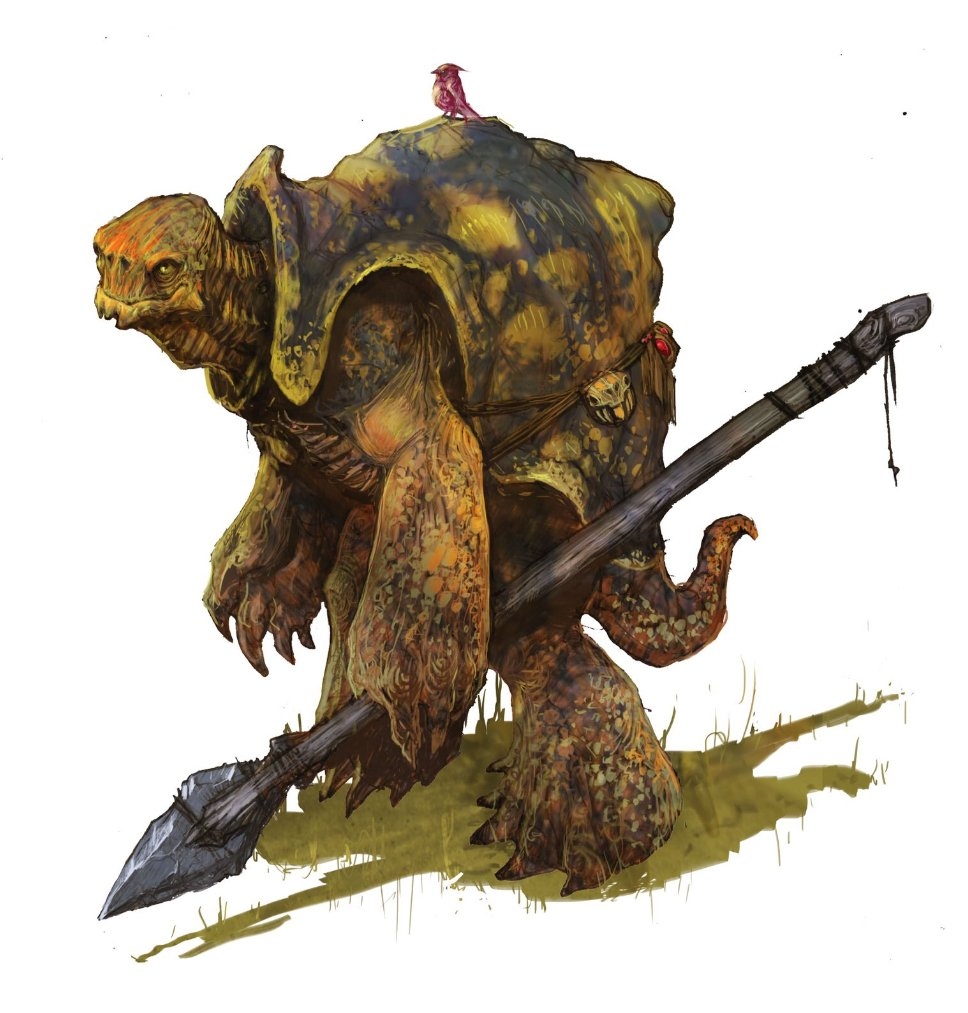
\includegraphics[width=0.48\textwidth]{03kins/img/tortle_official.jpg}
\end{figure}

\subsection*{Life of a Tortle}
A tortle hatches from a thick-shelled egg and spends the first few weeks of its life crawling on all fours.
Its parents usually leave soon after its birth, but spend what little time they have telling stories to their offspring. 
Within a year, the young tortle is abandoned and becomes an orphan, though not before it learns to speak and to survive on its own.

A young tortle and its siblings inherit whatever tools, weapons, and gifts their parents leave for them.
Each young tortle is expected to fend for itself.
It leaves the place of its birth and finds its own corner of the wilderness in which to hunt, catch fish, and get by.
With each passing year, a tortle hones its survival skills.
It forms friendships with its neighbors while also respecting their privacy.
At some point, a tortle feels an almost overwhelming urge to venture far away from home and see more of the world.
It gathers up its possessions and heads into the wilderness, returning months or years later with stories of its exploits and new skills.

Tortles are gendered creatures, and it is usual for them to seek out a mate and procreate when they return home from these travels.
Tortles lay their eggs (numbering as few as one or as many as a dozen) in a fortified compound enclosed by stone walls that are easily defensible.
If no such compound exists, they build one.
The parents spend the hatching time of their eggs guarding the compound and defending their offspring, and after they hatch they spend a year sharing their knowledge with the young ones.
The parents leave their children at this time, overburdened by their nomadic nature and confident that the older tortles of the village will care for them.
When the children are old enough to leave the compound, they pick up whatever weapons and tools their parents left behind and set out on their own.

\subsection*{Beliefs}
Tortles don't have a religion of their own, but they often worship the gods of other races.
It's not unusual for a tortle to hear stories or legends related to a god and choose to worship that deity.
Curious in nature, most tortles like to see how other creatures live and discover new customs and new ways of doing things.
Some tortles are also drawn to the many schools of thought, trying to learn from all of them instead of focusing on a single one.

Tortles believe that night and day watch over them and other creatures.
The moons are the eyes of night that watch over them in darkness, and the sun is the equally vigilant eye of day.
Tortles feel most at peace when these "eyes" are looking down on them.
They become more nervous and uneasy when no orb is visible in the sky.
Tortles tend to be most uncomfortable underground, where neither the sun nor the moons are visible to them.

Blessed are the days when many moons are visible in the sky at the same time.
Tortles often choose such days to leave their homes and begin a wilderness expedition, or perform some other task they know to be dangerous.

\subsection*{Inherent Mutualism}
Tortles have a special relationship to the anchelons.
Anchelons are colossal horned turtles that reside in Yuadrem's oceans, breeding fear among sailors and fishers alike.
They are generally fierce in nature but, while not sentient, they are oddly friendly toward tortles.
Anchelons lay their eggs in the beryl sea, and tortles allow thme to lay their eggs in their compounds.
It is not uncommon for baby anchelons to grow alongside tortles.
Anchelons in exchange protect the tortles' villages, and may even help tortles they encounter in the wilds.

\subsection*{Adventurers at Heart}
Tortles have a saying: "We wear our homes on our backs."
The shells they carry around provide all the shelter they require.
Consequently, tortles don't feel the need to root themselves in one place for too long.
A tortle settlement is primarily used as a kind of moot, where tortles can socialize with one another, share useful information, and trade with strangers in the safety of greater numbers.
Tortles don't regard these settlements as places worth defending with their lives, and they will abandon a settlement when it no longer serves their needs.

Tortles embrace a simple view of the world.
It is a place of wonder, and tortles see beauty in the ordinary.
They live for the chance to hear a soft wind blowing through palm trees, to watch a frog croaking on a lily pad, or to stand in a crowded marketplace.

Tortles like to learn new skills.
They craft their own tools and weapons, and they are good at building structures and fortifications.
They marvel at the works of other kins, and can lose themselves for years in a city, studying its architectural wonders and learning skills they can put to use when building forts to contain their offspring.

Although they spend a considerable portion of their lives in isolation, tortles are social creatures that like to form meaningful friendships.
Being native to another world, they have no inbred animus toward any kin.
In fact, a tortle will often seek out friendships with non-tortles to learn new customs and new points of view.

% \begin{figure}[!htbp]
%     \centering
%     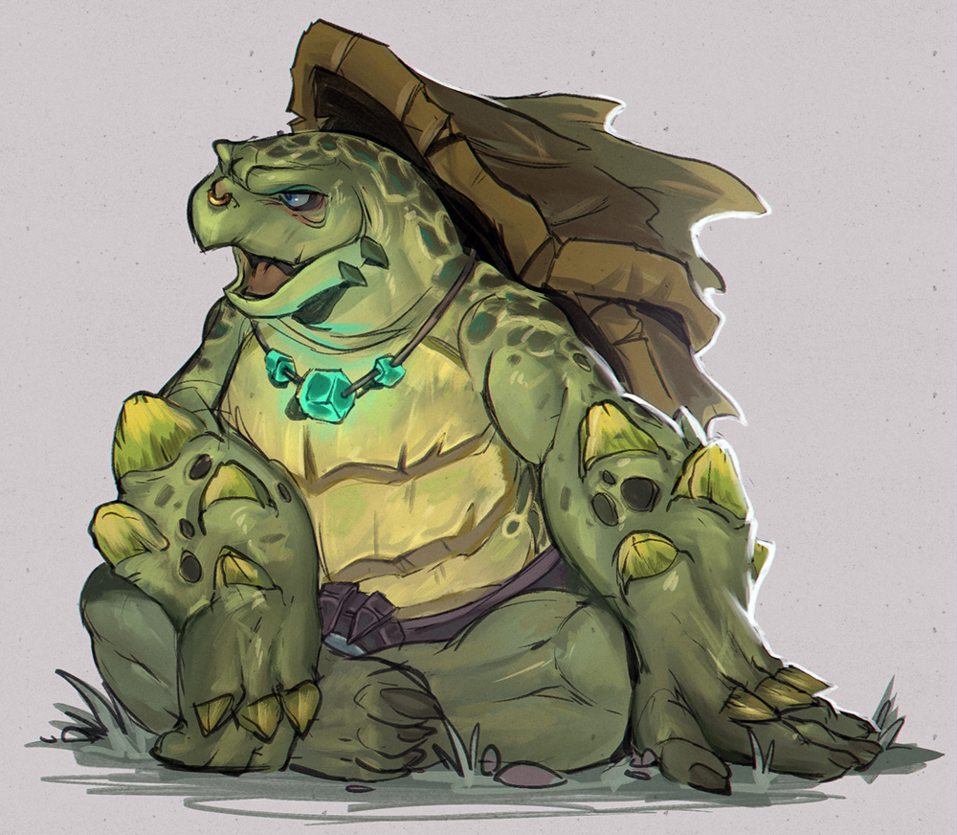
\includegraphics[width=0.48\textwidth]{03kins/img/tortle_chill.png}
% \end{figure}

\subsection*{Tortle Names}
Tortles prefer simple, non-gender-specific names that are usually no more than two syllables long.
If a tortle doesn't like its name for whatever reason, it can change it, and it might do this a dozen times in its life.

A tortle doesn't feel constrained by its name, which is designated only to refer to the tortle in contrast of its peers.
Tortles don't have surnames or family names.

\paragraph{Names}
Baka, Damu, Gar, Gura, Ini, Jappa, Kinlek, Krull, Lim, Lop, Nortle, Nulka, Olo, Ploqwat, Quee, Queg, Quott, Sunny, Tibor, Ubo, Uhok, Wabu, Xelbuk, Xopa, Yog

\subsection*{Traits}
Your tortle character gains traits that enable it to cope with the perils of a savage world.
\subparagraph{Ability Score Increase} Your Strength score increases by 2, and your Wisdom score increases by 1.
\subparagraph{Age} Young tortles crawl for a few weeks after birth before learning to walk on two legs. 
They reach adulthood by the age of 15 and live an average of 500 years.
\subparagraph{Alignment} Tortles tend to lead orderly, ritualistic lives.
They develop customs and routines, becoming more set in their ways as they age.
Most follow a set of tenets that the kin brought with them from the outer lands, leading to lawfulness.
While most are good, a few can be selfish and greedy, but it's unusual for a tortle to shuck off order in favor of chaos.
Tortles tend towards the gold tide, always empathic and helping others.
\subparagraph{Size} Tortle adults stand 1.5 to 1.8 meters tall and average 230 kg.
Their shells account for roughly one-third of their weight.
Your size is Medium.
\subparagraph{Claws} Your claws are natural weapons, which you can use to make unarmed strikes.
If you hit with them, you deal slashing damage equal to 1d4 + your Strength modifier, instead of bludgeoning damage normal for an unarmed strike.
\subparagraph{Hold Breath} Tortles aren't natural swimmers, but they can remain underwater for some time before needing to come up for air.
You can hold your breath for up to 1 hour at a time.
\subparagraph{Natural Armor} Due to your shell and the shape of your body, you are ill-suited to wearing armor.
Your shell provides ample protection, however; it gives you a base AC of 17 (your Dexterity modifier doesn't affect this number).
You gain no benefit from wearing armor, but if you are using a shield, you can apply the shield's bonus as normal.
\subparagraph{Shell Defense} You can withdraw into your shell as an action.
Until you emerge, you gain a +4 bonus to AC, and you have advantage on Strength and Constitution saving throws.
While in your shell, you are prone, your speed is 0 and can't increase, you have disadvantage on Dexterity saving throws, you can't take reactions, and the only action you can take is a bonus action to emerge from your shell.
\subparagraph{Survival Instinct} You gain proficiency in the Survival skill.
Tortles have finely honed survival instincts.
\subparagraph{Learned Tradition} You are proficient with two weapons, two sets of artisan's tools, or one of each of your choice.
This comes from the time spent with your parents, and you feel a special connection with these types of items.
\subparagraph{Languages} You can speak the krehlo tongue and one additional language of your choice, but cannot write or read either.
The krehlo tongue doesn't have a written form, and the tortle tenets are passed on in oral tradition.

\begin{table*}[b]%
    \begin{DndTable}[width=\linewidth]{X}
        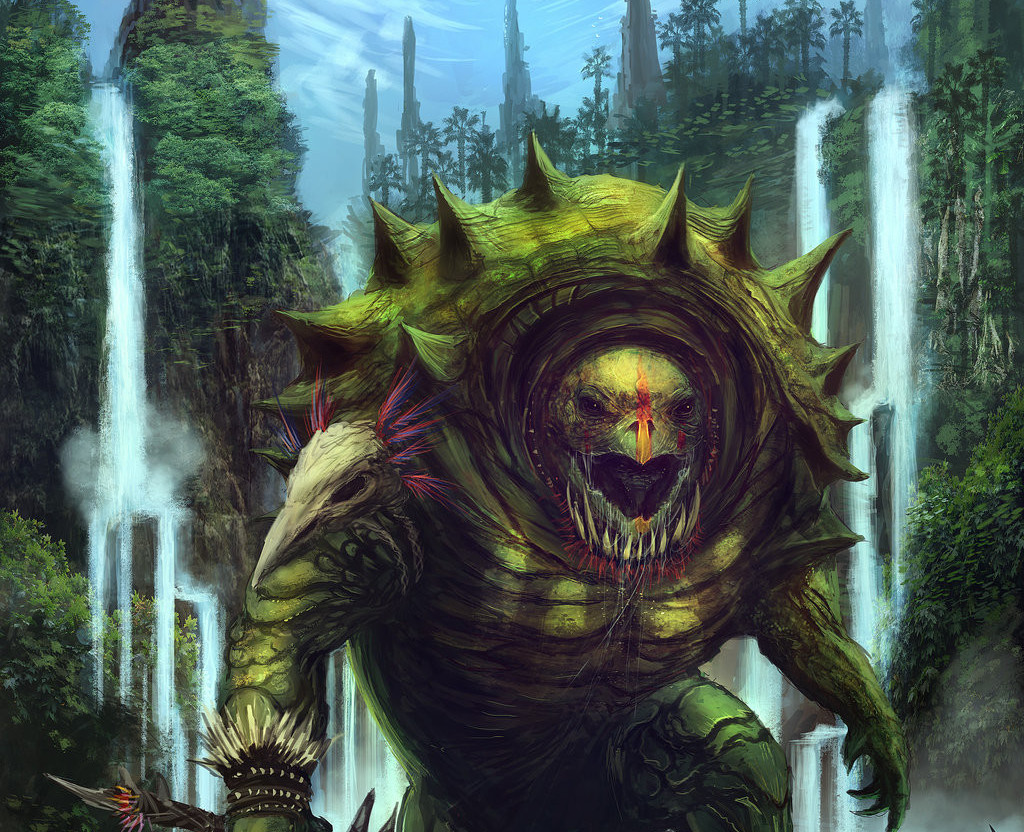
\includegraphics[width=0.98\textwidth]{03kins/img/tortle_spiked.jpg}
    \end{DndTable}
\end{table*}

\subsubsection{Steam Kin}
A very small proportion of the shelled kin population are born with special characteristics.
Their bodies are slightly larger and are of a stony appearance and color, their teeth are larger and sharper, and they have small growths on the top of their heads resembling tiny horns.
Their larger bodies prohibit them from nesting inside their shells.
They make up this lack of defense with a stronger offense however.
\subparagraph{Size} The steam kin are larger in nature than the average tortle.
Adults stand between 180 and 200 cm, and weigh on average 280 kg.
\subparagraph{Steam Breath} This trait replaces shell defense.
You can use your action to exhale a 20 feet cone of scalding steam.
Every target in the area must make a Dexterity saving throw, with a DC of (8 + your Constitution modifier + your proficiency bonus).
A creature takes 2d6 fire damage on a failed save, or half as much damage on a successful one.
The fire damage increases to 3d6 at 6th level, 4d6 at 11th level, and 5d6 at 16th level.
After you use this trait, you can't use it again until you complete a short or long rest.
Being underwater doesn't grant resistance to this damage.
\end{linenumbers}

\begin{DndSidebar}[float=!b]{Variant Tortle Trait}
    Being born of the communion of two beings, tortles present slight genetic differences based on their family trees.
    Tortles born in the settlements near Leeside possess one such difference, and are known to be born with a spiked shell.
    You can choose to replace your claws trait with impaling carapace.
    \subparagraph{Impaling Carapace} When you grapple a creature, the target takes 1d4 piercing damage if your grapple check succeeds.
    If another creature grapples you, they take 1d4 piercing damage.
    If you start your turn grappling or being grappled by a creature, it takes 1d4 piercing damage.
\end{DndSidebar}
